%% -*- coding:utf-8 -*-
\begin{figure}
\centering

\ifpdf
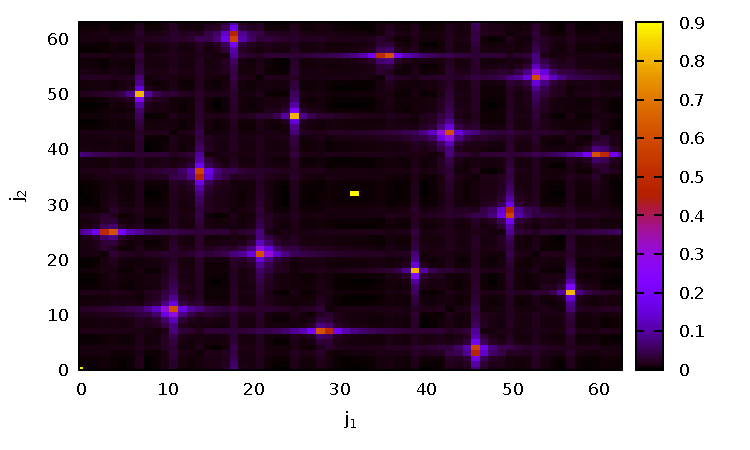
\includegraphics[angle=0]
{./part4/quantcomp/picdiscretlog3.pdf}
\else
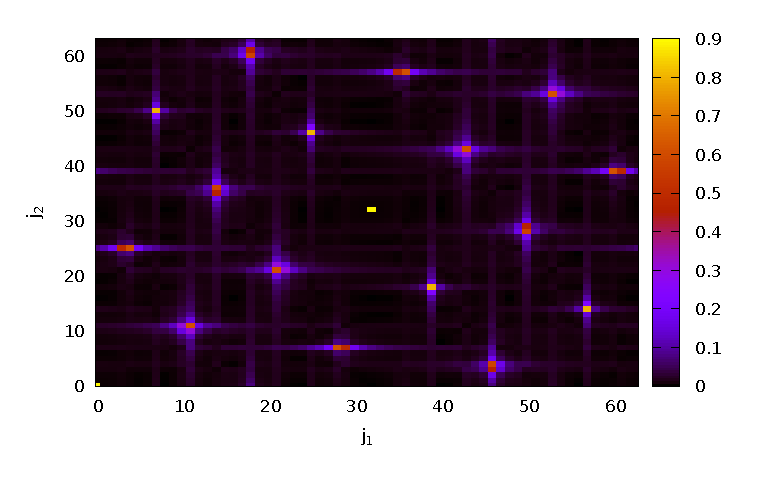
\includegraphics[angle=0]
{./part4/quantcomp/picdiscretlog3.eps}
\fi

%\input ./part4/quantcomp/picdiscretlog2.tex

\caption{Фурье образ отсчетов функции 
$f'(x_1, x_2)$
Число отсчетов $M=64$. Координаты максимума $j_1 \approx 46$, $j_2 \approx 3.5$. 
Решением уравнения $3^x \equiv 14 \mod 19$
является $x = 13 \approx \frac{46}{3.5} \approx 13.14$
} 
\label{fig:part4:quantcomp:dl3}
\end{figure}
